\documentclass[11pt,letterpaper]{article}

% --- Packages ---
\usepackage[margin=1in]{geometry}
\usepackage{setspace}
\usepackage{titlesec}
\usepackage{fancyhdr}
\usepackage{amsmath, amssymb,mathtools}
\usepackage{enumitem}
\usepackage{hyperref}
\usepackage{xcolor}
\usepackage{tcolorbox}
\usepackage{graphicx,wrapfig}
\usepackage[capitalize]{cleveref}

% --- Formatting ---
\setstretch{1.2}
\titleformat{\section}{\Large\bfseries}{\thesection.}{1em}{}
\titleformat{\subsection}{\large\bfseries}{\thesubsection}{1em}{}
\titleformat{\subsubsection}{\normalsize\bfseries}{\thesubsubsection}{1em}{}
\setlist[itemize]{topsep=2pt,itemsep=2pt,parsep=2pt,partopsep=2pt}

% --- Header/Footer ---
\pagestyle{fancy}
\fancyhf{}
\lhead{Course: \textbf{Machine Learning Specialization}}
\rhead{\textbf{Nov 2025}}
\cfoot{\thepage}

% --- Custom Note Boxes ---
\newtcolorbox{definitionbox}{
  colback=blue!5!white,
  colframe=blue!75!black,
  title=Definition
}

\newtcolorbox{theorembox}{
  colback=green!5!white,
  colframe=green!60!black,
  title=Theorem
}

\newtcolorbox{examplebox}{
  colback=orange!5!white,
  colframe=orange!85!black,
  title=Example
}

\newtcolorbox{notebox}{
  colback=yellow!10!white,
  colframe=yellow!50!black,
  title=Note
}

% --- Document ---
\begin{document}

\begin{center}
    {\LARGE \textbf{Course 2 Notes: Advanced Learning Algorithms}}\\[0.5em]
    {\large Adrew Ng\quad | \quad Jesse Hernandez}\\[0.25em]
    {\small DeepLearningAI/Stanford Online\quad | \quad 2025}
\end{center}

\vspace{1em}
\hrule
\vspace{1em}

{\noindent\Large \color{blue} My notes for the second course in a three part machine learning specialization course on coursera consisting of four learning modules.}

% --- Example Lecture Outline ---
\section{Week 1: Neural Networks}

\subsection{Overview}

- Key objectives  
\begin{itemize}
	\item Introduction to Neural Networks
	\item Nueral Network Training
	\item Practical advice on building ML systems
	\item Decision Trees
\end{itemize}

\noindent 
- Background context  
\begin{itemize}
	\item Building Neural network from scratch and with Tensorflow for inference and training
\end{itemize}

\subsubsection{Neurons as inspiration}

\begin{notebox}
	\begin{itemize}[leftmargin=*]
		\item The origins of neural networks were to build algorithms that mimicked the brain
		\item Re-popularized in 2005 in the category of Deep Leaning
		\item Initially successful in speech recognition then image recognition followed by Natural Language Processing (NLP) and now used in many more applications
		\item Biological neurons function by taking many electrical impulses as inputs and outputs the response to send to the next neuron until it reaches the brain 
		\item Neural Networks saw huge performance improvements particularly with Big Data,e.g., performance scales with amount of data,  
	\end{itemize}
\end{notebox}

\subsection{Introduction to Neural Networks}

\begin{definitionbox}
	A \textbf{Neural Network} is a type of machine learning inspired by how the brain works using layered structure of interconnected nodes or 'neurons' to process data, recognize patterns and make predictions.
\end{definitionbox}

\begin{examplebox}
	\textbf{Demand Prediction} example using neural network.
	\begin{itemize}
		\item We are trying to predict the probability of being a top seller for clothing product
		\item The inputs or features to the model are price, shipping cost, marketing, and material (input layer)
		\item The criteria (\textbf{activations}) are affordability, awareness, and perceived quality (forms the nodes of our neural layer or \textbf{hidden layer} that outputs \textbf{activation values})
		\item Relevant features map out to different nodes to access its criteria ranking, in practice the network will find the best features to use (analogous to automated feature engineering)
		\item All outputs from the layer is fed to another node (output layer) to process the probability of being a top seller 
		\item the independent nodes each run independent logistic regression (input model) algorithms to output probabilities 
		\item Simple to vectorize inputs and outputs of to run through layers and come to a prediction, here $\vec{x},\ \vec{a}$ are the inputs and activation values respectively,
		\[ \vec{x}\rightarrow \textbf{(hidden layer)}\rightarrow \vec{a}\rightarrow \textbf{(output layer)}\rightarrow a  \]
	\end{itemize}
	
	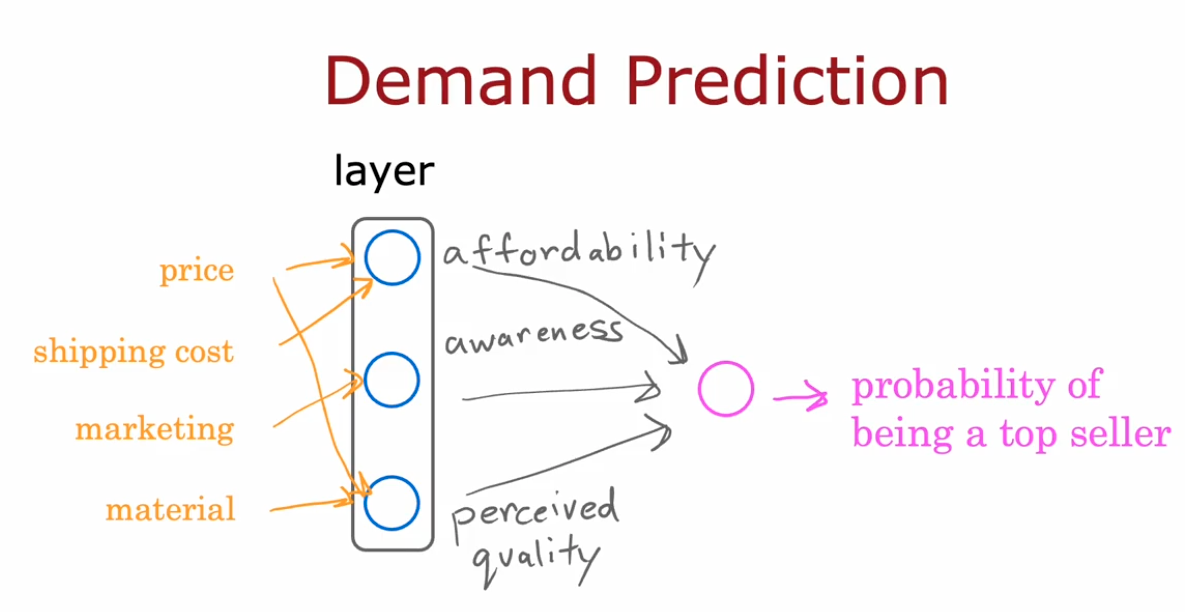
\includegraphics[height=6cm]{course_img/neural_network_ex}
\end{examplebox}

\begin{notebox}
	\begin{itemize}[leftmargin=*]
		\item Depending on the \textbf{neural network architecture} there can be many hidden layers with different number of nodes in each (\textbf{multilayer perceptron})
		\item choosing how to construct the neural network depending on what problem you have can affect performance and accuracyand will be discussed in week 3
	\end{itemize}
\end{notebox}

\subsubsection{Recognizing Images}

\begin{examplebox}
	\textbf{Face recognition} problem is to identify the person in the image using the pixel data of the image
	\begin{itemize}
		\item The image data is read as a $m\times n$ matrix of pixel intensities
		\item The input features are then these values rolled out into a vector of  $m\times n$ length,e.g., a 1000x1000 pixel image will have 1 million pixel intensity features as input to the network
		\item Shown below is how many hidden layers may naturally break the task into pieces at each layer with different imgae scopes and aggregate the information to get a probability for being person XYZ
		\begin{enumerate}
			\item Layer 1 may look for edges or shapes (fine scope)
			\item Layer two may take layer 1 input to find facial structures, e.g., eyes,nose, etc (medium scope)
			\item Layer 3 may agregate the facial features to form full facial images (large scope)
		\end{enumerate}
	\end{itemize}
	
	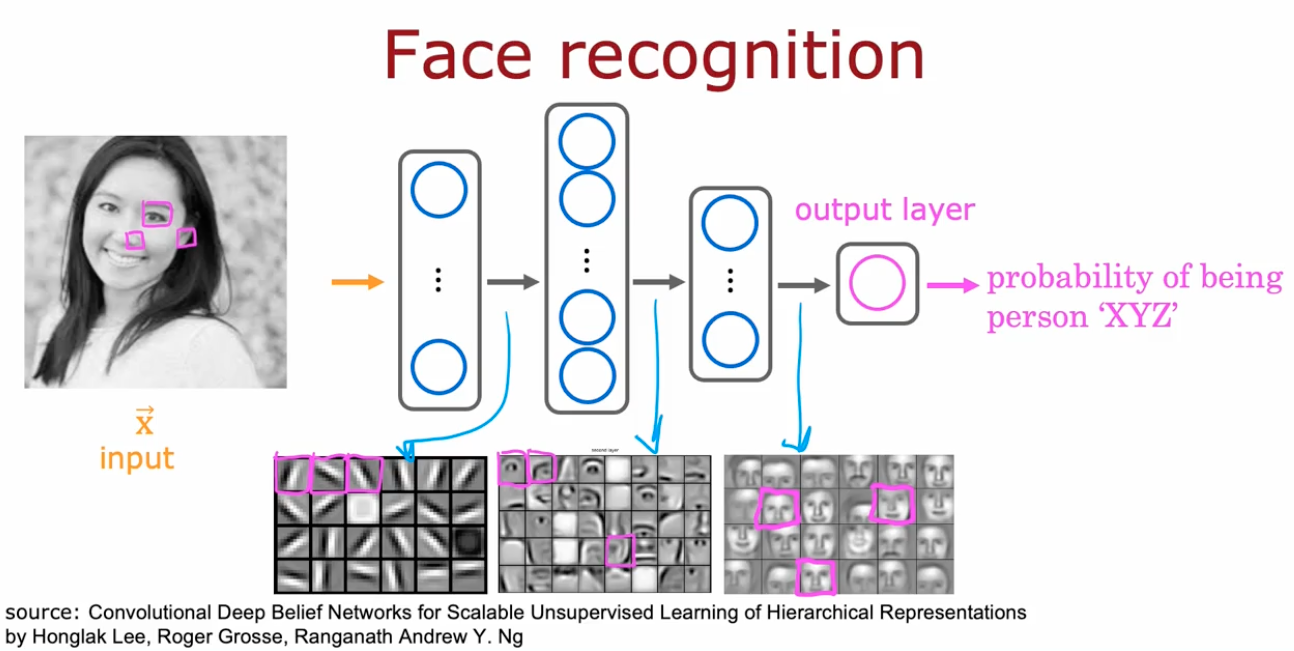
\includegraphics[height=6cm]{course_img/face_recognition_ex}
\end{examplebox}

\begin{notebox}
	The neural network can be tasked to find cars and the layers will automatically learn to search for car features.  
\end{notebox}	

\subsection{Neural Networks in action}

\begin{definitionbox}
	The \textbf{neural network layer} is composed of many nodes ($n_1\dots n_i$) taking in all the features $\vec{x}$ with parameters optimized for each node ($\vec{w}_i,\ b_i$) from the set of features and outputs the activation value for each node $a_i$, which forms the activation vector(hidden layer output) $\vec{a}$. 
	\begin{itemize}
		\item Each node is running a logistic regression model such that $a_i = g(z)$ where the definitions for the regression model $z$ (linear or polynomial)  is transformed using a sigmoid ($g(z)$) function discussed in course 1. 
		\item For multi-layer neural networks we will use the superscript notation $\vec{a}^{[ j ]}$ to denote the $j$\textsuperscript{th}~layer
		\item The activation values of each layer $\vec{a}^{[ j ]}$ then become the input values for the subsequent layer 
	\end{itemize}
\end{definitionbox}

\begin{examplebox}
	An example of a more complex neutral network may look like this (below), where the calculation for the third hidden layer using a logisitc regression transforamtion of a linear regression model:\\
	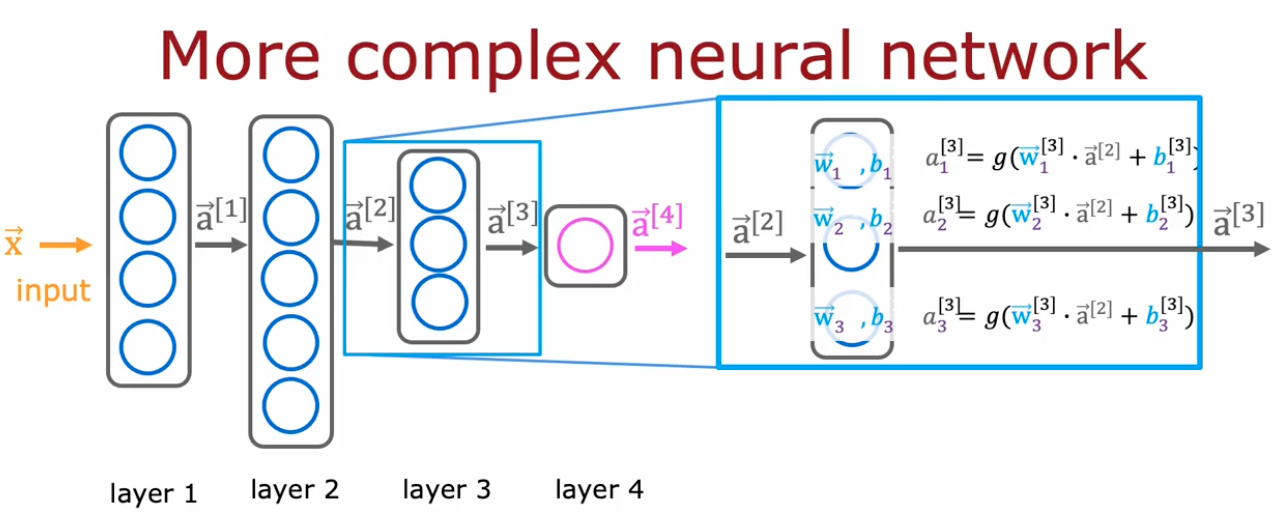
\includegraphics[width=\textwidth]{course_img/complex_NN_ex}
	
	\begin{itemize}[leftmargin=*]
		\item The third layer calculations are using the second layer outputs: $a^{[3]}_i = g(\vec{w}^{[3]}_i\cdot \vec{a}^{[2]} + b_i^{[3]})$ 
	\end{itemize}
	
	This can be generalized for logistic regression with a linear regression model as:
	\begin{equation}\label{eq:NN_activation_value}
		a_j^{[l]} = g(\vec{w}^{[l]}_j\cdot \vec{a}^{[l - 1]} + b_j^{[l]}),
	\end{equation}
	where $l$ is the layer number and $j$ is the node number.  Here $g(z)$ is the \textbf{activation function} and can take other forms but is a sigmoid function here.
\end{examplebox}

\subsubsection{Inference: making predictions}

\begin{definitionbox}
	\textbf{Forward propagation} is a machine learning algorithm used with neural networks to make predictions by propagating the results forward through the hidden layers to the output value (see example below)
	\begin{itemize}
		\item Forward propagation can be used to predict values using an existing neural network with tuned parameters,  in the next lesson we will learn to train our own neural network 
	\end{itemize}
\end{definitionbox}

\begin{examplebox}
	\textbf{Handwritten digit recognition} example is shown below where we want to find teh porbability of the image being a one and take an 8 x 8 pixel image as input with 2 hidden layers having 25 and 15 nodes\\
	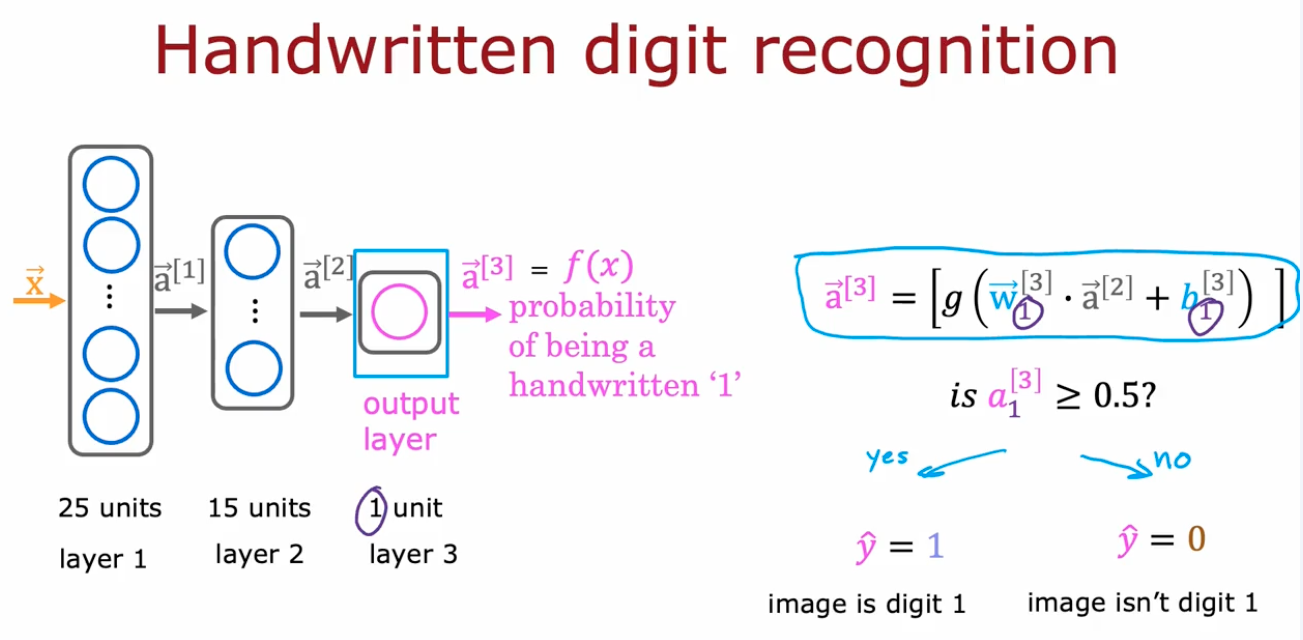
\includegraphics[width=\textwidth]{course_img/hadwritten_NN_ex}
	
	\begin{itemize}[leftmargin=*]
		\item The image above shows only the computation for the final output layer, more generally each activation vector is solved:
			\begin{equation}
				\vec{a}^{[l]}=
				\begin{bmatrix}
					g(\vec{w}^{[l]}_1\cdot \vec{a}^{[l - 1]} + b_j^{[l]}) \\
					\vdots \\
					g(\vec{w}^{[l]}_j\cdot \vec{a}^{[l - 1]} + b_j^{[l]})
				\end{bmatrix}
			\end{equation}
	\end{itemize}
\end{examplebox}

\subsection{Implementations}

-- Neural network implementation in Tensorflow (Lab 1).

-- Neural network implementation from scratch using Numpy (Lab 2)

-- Matrix implementation for efficient vectorization for implementation

\section{Week 2: Neural Network Training}


\end{document}